\documentclass[12pt,a4paper,]{book}
\def\ifdoblecara{} %% set to true
\def\ifprincipal{} %% set to true
\def\ifcitapandoc{} %% set to true
\let\ifcitapandoc\undefined %% set to false
\usepackage{lmodern}
\usepackage{amssymb,amsmath}
\usepackage{ifxetex,ifluatex}
%\usepackage{fixltx2e} % provides \textsubscript %PLLC
\ifnum 0\ifxetex 1\fi\ifluatex 1\fi=0 % if pdftex
  \usepackage[T1]{fontenc}
  \usepackage[utf8]{inputenc}
\else % if luatex or xelatex
  \ifxetex
    \usepackage{mathspec}
  \else
    \usepackage{fontspec}
  \fi
  \defaultfontfeatures{Ligatures=TeX,Scale=MatchLowercase}
\fi
% use upquote if available, for straight quotes in verbatim environments
\IfFileExists{upquote.sty}{\usepackage{upquote}}{}
% use microtype if available
\IfFileExists{microtype.sty}{%
\usepackage{microtype}
\UseMicrotypeSet[protrusion]{basicmath} % disable protrusion for tt fonts
}{}
\usepackage[margin = 2.5cm]{geometry}
\usepackage{hyperref}
\hypersetup{unicode=true,
              pdfborder={0 0 0},
              breaklinks=true}
\urlstyle{same}  % don't use monospace font for urls
\usepackage{natbib}
\bibliographystyle{apalike}
%%% desaptivado lo que sigue
%\usepackage[usenames,dvipsnames]{xcolor}  %new PLLC
\usepackage{longtable,booktabs}
\IfFileExists{parskip.sty}{%
\usepackage{parskip}
}{% else
\setlength{\parindent}{0pt}
\setlength{\parskip}{6pt plus 2pt minus 1pt}
}
\setlength{\emergencystretch}{3em}  % prevent overfull lines
\providecommand{\tightlist}{%
  \setlength{\itemsep}{0pt}\setlength{\parskip}{0pt}}
\setcounter{secnumdepth}{5}
% Redefines (sub)paragraphs to behave more like sections
\ifx\paragraph\undefined\else
\let\oldparagraph\paragraph
\renewcommand{\paragraph}[1]{\oldparagraph{#1}\mbox{}}
\fi
\ifx\subparagraph\undefined\else
\let\oldsubparagraph\subparagraph
\renewcommand{\subparagraph}[1]{\oldsubparagraph{#1}\mbox{}}
\fi

%%% Use protect on footnotes to avoid problems with footnotes in titles
\let\rmarkdownfootnote\footnote%
\def\footnote{\protect\rmarkdownfootnote}


  \title{}
    \author{}
    \date{}
  

%%%%%%% inicio: latex_preambulo.tex PLLC

%% UTILIZA CODIFICACIÓN UTF-8
%% MODIFICARLO CONVENIENTEMENTE PARA USARLO CON OTRAS CODIFICACIONES


%\usepackage[spanish,es-nodecimaldot,es-noshorthands]{babel}
\usepackage[spanish,es-nodecimaldot,es-noshorthands,es-tabla]{babel}
% Ver: es-tabla (en: https://osl.ugr.es/CTAN/macros/latex/contrib/babel-contrib/spanish/spanish.pdf)
% es-tabla (en: https://tex.stackexchange.com/questions/80443/change-the-word-table-in-table-captions)
\usepackage{float}
\usepackage{placeins}
\usepackage{fancyhdr}   %desaptivado por mí
% Solucion: ! LaTeX Error: Command \counterwithout already defined.
% https://tex.stackexchange.com/questions/425600/latex-error-command-counterwithout-already-defined
\let\counterwithout\relax
\let\counterwithin\relax
\usepackage{chngcntr}
%\usepackage{microtype}  %antes en template PLLC
\usepackage[utf8]{inputenc}
\usepackage[T1]{fontenc} % Usa codificación 8-bit que tiene 256 glyphs

%\usepackage[dvipsnames]{xcolor}
%\usepackage[usenames,dvipsnames]{xcolor}  %new
\usepackage{pdfpages}
%\usepackage{natbib}




% Para portada: latex_paginatitulo_mod_ST02.tex (inicio)
\usepackage{tikz}
\usepackage{epigraph}
\renewcommand\epigraphflush{flushright}
\renewcommand\epigraphsize{\normalsize}
\setlength\epigraphwidth{0.7\textwidth}

\definecolor{titlepagecolor}{cmyk}{1,.60,0,.40}

%\DeclareFixedFont{\titlefont}{T1}{ppl}{b}{it}{0.5in}

% \makeatletter
% \def\printauthor{%
%     {\large \@author}}
% \makeatother
% \author{%
%     Author 1 name \\
%     Department name \\
%     \texttt{email1@example.com}\vspace{20pt} \\
%     Author 2 name \\
%     Department name \\
%     \texttt{email2@example.com}
%     }

% The following code is borrowed from: https://tex.stackexchange.com/a/86310/10898

\newcommand\titlepagedecoration{%
\begin{tikzpicture}[remember picture,overlay,shorten >= -10pt]

\coordinate (aux1) at ([yshift=-15pt]current page.north east);
\coordinate (aux2) at ([yshift=-410pt]current page.north east);
\coordinate (aux3) at ([xshift=-4.5cm]current page.north east);
\coordinate (aux4) at ([yshift=-150pt]current page.north east);

\begin{scope}[titlepagecolor!40,line width=12pt,rounded corners=12pt]
\draw
  (aux1) -- coordinate (a)
  ++(225:5) --
  ++(-45:5.1) coordinate (b);
\draw[shorten <= -10pt]
  (aux3) --
  (a) --
  (aux1);
\draw[opacity=0.6,titlepagecolor,shorten <= -10pt]
  (b) --
  ++(225:2.2) --
  ++(-45:2.2);
\end{scope}
\draw[titlepagecolor,line width=8pt,rounded corners=8pt,shorten <= -10pt]
  (aux4) --
  ++(225:0.8) --
  ++(-45:0.8);
\begin{scope}[titlepagecolor!70,line width=6pt,rounded corners=8pt]
\draw[shorten <= -10pt]
  (aux2) --
  ++(225:3) coordinate[pos=0.45] (c) --
  ++(-45:3.1);
\draw
  (aux2) --
  (c) --
  ++(135:2.5) --
  ++(45:2.5) --
  ++(-45:2.5) coordinate[pos=0.3] (d);   
\draw 
  (d) -- +(45:1);
\end{scope}
\end{tikzpicture}%
}

% Para portada: latex_paginatitulo_mod_ST02.tex (fin)

% Para portada: latex_paginatitulo_mod_OV01.tex (inicio)
\usepackage{cpimod}
% Para portada: latex_paginatitulo_mod_OV01.tex (fin)

% Para portada: latex_paginatitulo_mod_OV03.tex (inicio)
\usepackage{KTHEEtitlepage}
% Para portada: latex_paginatitulo_mod_OV03.tex (fin)

\renewcommand{\contentsname}{Índice}
\renewcommand{\listfigurename}{Índice de figuras}
\renewcommand{\listtablename}{Índice de tablas}
\newcommand{\bcols}{}
\newcommand{\ecols}{}
\newcommand{\bcol}[1]{\begin{minipage}{#1\linewidth}}
\newcommand{\ecol}{\end{minipage}}
\newcommand{\balertblock}[1]{\begin{alertblock}{#1}}
\newcommand{\ealertblock}{\end{alertblock}}
\newcommand{\bitemize}{\begin{itemize}}
\newcommand{\eitemize}{\end{itemize}}
\newcommand{\benumerate}{\begin{enumerate}}
\newcommand{\eenumerate}{\end{enumerate}}
\newcommand{\saltopagina}{\newpage}
\newcommand{\bcenter}{\begin{center}}
\newcommand{\ecenter}{\end{center}}
\newcommand{\beproof}{\begin{proof}} %new
\newcommand{\eeproof}{\end{proof}} %new
%De: https://texblog.org/2007/11/07/headerfooter-in-latex-with-fancyhdr/
% \fancyhead
% E: Even page
% O: Odd page
% L: Left field
% C: Center field
% R: Right field
% H: Header
% F: Footer
%\fancyhead[CO,CE]{Resultados}

%OPCION 1
% \fancyhead[LE,RO]{\slshape \rightmark}
% \fancyhead[LO,RE]{\slshape \leftmark}
% \fancyfoot[C]{\thepage}
% \renewcommand{\headrulewidth}{0.4pt}
% \renewcommand{\footrulewidth}{0pt}

%OPCION 2
% \fancyhead[LE,RO]{\slshape \rightmark}
% \fancyfoot[LO,RE]{\slshape \leftmark}
% \fancyfoot[LE,RO]{\thepage}
% \renewcommand{\headrulewidth}{0.4pt}
% \renewcommand{\footrulewidth}{0.4pt}
%%%%%%%%%%
\usepackage{calc,amsfonts}
% Elimina la cabecera de páginas impares vacías al finalizar los capítulos
\usepackage{emptypage}
\makeatletter

\definecolor{ocre}{RGB}{25,25,243} % Define el color naranja usado para resaltar algunas salidas

%\usepackage{calc} 

\usepackage{lipsum}

%\usepackage{tikz} % Requerido para dibujar formas personalizadas

%\usepackage{amsmath,amsthm,amssymb,amsfonts}
\usepackage{amsthm}

%%%%%%% DE TEOREMAS %%%%%%%%%%
% Boxed/framed environments
\newtheoremstyle{ocrenumbox}% % Theorem style name
{0pt}% Space above
{0pt}% Space below
{\normalfont}% % Body font
{}% Indent amount
%%% Descomentado por mí , letra bf: de teoremas,def,ejemplos
{\small\bf\sffamily\color{ocre}}% % Theorem head font
{\;}% Punctuation after theorem head
{0.25em}% Space after theorem head
{\small\sffamily\color{ocre}\thmname{#1}\nobreakspace\thmnumber{\@ifnotempty{#1}{}\@upn{#2}}% Theorem text (e.g. Theorem 2.1)
%%%% \bfseries: bf para textos de: teoremas,definiciones, ejemplos
\thmnote{\nobreakspace\the\thm@notefont\sffamily\bfseries\color{black}---\nobreakspace#3.}} % Optional theorem note
\renewcommand{\qedsymbol}{$\blacksquare$}% Optional qed square

\newtheoremstyle{blacknumex}% Theorem style name
{5pt}% Space above
{5pt}% Space below
{\normalfont}% Body font
%{\textit}% Body font
{} % Indent amount
%%% Descomentado por mí 
%{\small\bf\sffamily}% Theorem head font
{\small\bf\sffamily}% Theorem head font
{\;}% Punctuation after theorem head
{0.25em}% Space after theorem head
{\small\sffamily{\tiny\ensuremath{\blacksquare}}\nobreakspace\thmname{#1}\nobreakspace\thmnumber{\@ifnotempty{#1}{}\@upn{#2}}% Theorem text (e.g. Theorem 2.1)
\thmnote{\nobreakspace\the\thm@notefont\sffamily\bfseries---\nobreakspace#3.}}% Optional theorem note

\newtheoremstyle{blacknumbox} % Theorem style name
{0pt}% Space above
{0pt}% Space below
{\normalfont}% Body font
%{\textit}% Body font
{}% Indent amount
%%% Descomentado por mí 
%{\small\bf\sffamily}% Theorem head font
{\small\bf\sffamily}% Theorem head font
{\;}% Punctuation after theorem head
{0.25em}% Space after theorem head
{\small\sffamily\thmname{#1}\nobreakspace\thmnumber{\@ifnotempty{#1}{}\@upn{#2}}% Theorem text (e.g. Theorem 2.1)
\thmnote{\nobreakspace\the\thm@notefont\sffamily\bfseries---\nobreakspace#3.}}% Optional theorem note

% Non-boxed/non-framed environments
\newtheoremstyle{ocrenum}% % Theorem style name
{5pt}% Space above
{5pt}% Space below
{\normalfont}% % Body font
%{\textit}% Body font
{}% Indent amount
%%% Descomentado por mí 
%{\small\bf\sffamily\color{ocre}}% % Theorem head font
{\small\bf\sffamily\color{ocre}}% % Theorem head font
{\;}% Punctuation after theorem head
{0.25em}% Space after theorem head
{\small\sffamily\color{ocre}\thmname{#1}\nobreakspace\thmnumber{\@ifnotempty{#1}{}\@upn{#2}}% Theorem text (e.g. Theorem 2.1)
\thmnote{\nobreakspace\the\thm@notefont\sffamily\bfseries\color{black}---\nobreakspace#3.}} % Optional theorem note
\renewcommand{\qedsymbol}{$\blacksquare$}% Optional qed square
\makeatother


% Define el estilo del texto theorem para cada tipo definido anteriormente
\newcounter{dummy} 
\numberwithin{dummy}{section}
\theoremstyle{ocrenumbox}

\newtheorem{theoremeT}[dummy]{Teorema}  % (Pedro: Theorem)

\newtheorem{problem}{Problema}[chapter]  % (Pedro: Problem)

\newtheorem{exerciseT}{Ejercicio}[chapter] % (Pedro: Exercise)

%%%%%%%%%%% color texto ejemplos
\theoremstyle{ocrenumbox}
\newtheorem{exampleT}{Ejemplo}[chapter] % (Pedro: Example)

\theoremstyle{ocrenumbox}

\newtheorem{vocabulary}{Vocabulario}[chapter]  % (Pedro: Vocabulary)

\newtheorem{definitionT}{Definición}[section]  % (Pedro: Definition)
\newtheorem{corollaryT}[dummy]{Corolario}  % (Pedro: Corollary)
\theoremstyle{ocrenumbox}
\newtheorem{proposition}[dummy]{Proposición} % (Pedro: Proposition)

\usepackage[framemethod=default]{mdframed}


\newcommand{\intoo}[2]{\mathopen{]}#1\,;#2\mathclose{[}}
\newcommand{\ud}{\mathop{\mathrm{{}d}}\mathopen{}}
\newcommand{\intff}[2]{\mathopen{[}#1\,;#2\mathclose{]}}
\newtheorem{notation}{Notation}[chapter]


%\mdfdefinestyle{exampledefault}{%
%rightline=true,innerleftmargin=10,innerrightmargin=10,
%frametitlerule=true,frametitlerulecolor=green,
%frametitlebackgroundcolor=yellow,
%frametitlerulewidth=2pt}


% Theorem box
\newmdenv[skipabove=7pt,
skipbelow=7pt,
%backgroundcolor=black!5,
rightline=false,
leftline=false,
topline=false,
bottomline=false,
linecolor=gray,
%backgroundcolor=black!5,
innerleftmargin=5pt,
innerrightmargin=5pt,
innertopmargin=10pt,%5pt
leftmargin=0cm,
rightmargin=0cm,
linewidth=0pt,
innerbottommargin=0pt]{tBox}

% Exercise box	  
\newmdenv[skipabove=7pt,
skipbelow=7pt,
rightline=false,
leftline=true,
topline=false,
bottomline=false,
backgroundcolor=ocre!10,
linecolor=ocre,
innerleftmargin=5pt,
innerrightmargin=5pt,
innertopmargin=10pt,%5pt
innerbottommargin=5pt,
leftmargin=0cm,
rightmargin=0cm,
linewidth=4pt]{eBox}	

% Definition box
\newmdenv[skipabove=7pt,
skipbelow=7pt,
rightline=false,
leftline=false,
topline=false,
bottomline=false,
%backgroundcolor=black!5,
linecolor=gray,
innerleftmargin=5pt,
innerrightmargin=5pt,
innertopmargin=10pt,%0pt
leftmargin=0cm,
rightmargin=0cm,
linewidth=0pt,
innerbottommargin=0pt]{dBox}	

% Corollary box
\newmdenv[skipabove=7pt,
skipbelow=7pt,
rightline=false,
leftline=true,
topline=false,
bottomline=false,
linecolor=gray,
backgroundcolor=black!5,
innerleftmargin=5pt,
innerrightmargin=5pt,
innertopmargin=10pt,%5pt
leftmargin=0cm,
rightmargin=0cm,
linewidth=5pt,
innerbottommargin=5pt]{cBox}

%%% nuevo ejemplo
% example box
\newmdenv[skipabove=7pt,
skipbelow=7pt,
rightline=false,
leftline=false,
topline=false,
bottomline=false,
%backgroundcolor=black!5,
linecolor=gray,
innerleftmargin=5pt,
innerrightmargin=5pt,
innertopmargin=10pt,%0pt
leftmargin=0cm,
rightmargin=0cm,
linewidth=0pt,
innerbottommargin=0pt]{exBox}	



% Crea un entorno para cada tipo de theorem y le asigna un estilo 
% con ayuda de las cajas coloreadas anteriores

%\newenvironment{theorem}{\begin{tBox}\begin{theoremeT}}{\end{theoremeT}\end{tBox}}

\newenvironment{exercise}{\begin{eBox}\begin{exerciseT}}{\hfill{\color{ocre}\tiny\ensuremath{\blacksquare}}\end{exerciseT}\end{eBox}}				  
%\newenvironment{definition}{\begin{dBox}\begin{definitionT}}{\end{definitionT}\end{dBox}}	

%%%% Cuadrado negro al final de: teorema, definicion, ejemplos

\newenvironment{theorem}{\begin{theoremeT}}{\hfill{\small\ensuremath{\blacksquare}}\end{theoremeT}}		

\newenvironment{example}{\begin{exampleT}}{\hfill{\small\ensuremath{\blacksquare}}\end{exampleT}}		

\newenvironment{definition}{\begin{definitionT}}{\hfill{\small\ensuremath{\blacksquare}}\end{definitionT}}		


%%%%%% nuevo ejemplo
%\newenvironment{example}{\begin{exBox}\begin{exampleT}}{\end{exampleT}\end{exBox}}	

\newenvironment{corollary}{\begin{cBox}\begin{corollaryT}}{\end{corollaryT}\end{cBox}}	

%	ENVIRONMENT remark
\newenvironment{remark}{\par\vspace{10pt}\small 
% Espacio blanco vertical sobre la nota y tamaño de fuente menor
\begin{list}{}{
\leftmargin=35pt % Indentación sobre la izquierda
\rightmargin=25pt}\item\ignorespaces % Indentación sobre la derecha
\makebox[-2.5pt]{\begin{tikzpicture}[overlay]
\node[draw=ocre!60,line width=1pt,circle,fill=ocre!25,font=\sffamily\bfseries,inner sep=2pt,outer sep=0pt] at (-15pt,0pt){\textcolor{ocre}{N}}; \end{tikzpicture}} % R naranja en un círculo (Pedro)
\advance\baselineskip -1pt}{\end{list}\vskip5pt} 
% Espaciado de línea más estrecho y espacio en blanco después del comentario


\newenvironment{solutionExe}{\par\vspace{10pt}\small 
\begin{list}{}{
\leftmargin=35pt 
\rightmargin=25pt}\item\ignorespaces 
\makebox[-2.5pt]{\begin{tikzpicture}[overlay]
\node[draw=ocre!60,line width=1pt,circle,fill=ocre!25,font=\sffamily\bfseries,inner sep=2pt,outer sep=0pt] at (-15pt,0pt){\textcolor{ocre}{S}}; \end{tikzpicture}} 
\advance\baselineskip -1pt}{\end{list}\vskip5pt} 

\newenvironment{solutionExa}{\par\vspace{10pt}\small 
\begin{list}{}{
\leftmargin=35pt 
\rightmargin=25pt}\item\ignorespaces 
\makebox[-2.5pt]{\begin{tikzpicture}[overlay]
\node[draw=ocre!60,line width=1pt,circle,fill=ocre!55,font=\sffamily\bfseries,inner sep=2pt,outer sep=0pt] at (-15pt,0pt){\textcolor{ocre}{S}}; \end{tikzpicture}} 
\advance\baselineskip -1pt}{\end{list}\vskip5pt} 

\usepackage{tcolorbox}

\usetikzlibrary{trees}

\theoremstyle{ocrenum}
\newtheorem{solutionT}[dummy]{Solución}  % (Pedro: Corollary)
\newenvironment{solution}{\begin{cBox}\begin{solutionT}}{\end{solutionT}\end{cBox}}	


\newcommand{\tcolorboxsolucion}[2]{%
\begin{tcolorbox}[colback=green!5!white,colframe=green!75!black,title=#1] 
 #2
 %\tcblower  % pone una línea discontinua
\end{tcolorbox}
}% final definición comando

\newtcbox{\mybox}[1][green]{on line,
arc=0pt,outer arc=0pt,colback=#1!10!white,colframe=#1!50!black, boxsep=0pt,left=1pt,right=1pt,top=2pt,bottom=2pt, boxrule=0pt,bottomrule=1pt,toprule=1pt}


%\mdfdefinestyle{exampledefault}{%
%rightline=true,innerleftmargin=10,innerrightmargin=10,
%frametitlerule=true,frametitlerulecolor=green,
%frametitlebackgroundcolor=yellow,
%frametitlerulewidth=2pt}



\newcommand{\betheorem}{\begin{theorem}}
\newcommand{\eetheorem}{\end{theorem}}

\newcommand{\bedefinition}{\begin{definition}}
\newcommand{\eedefinition}{\end{definition}}

\newcommand{\beremark}{\begin{remark}}
\newcommand{\eeremark}{\end{remark}}

\newcommand{\beexercise}{\begin{exercise}}
\newcommand{\eeexercise}{\end{exercise}}

\newcommand{\beexample}{\begin{example}}
\newcommand{\eeexample}{\end{example}}

\newcommand{\becorollary}{\begin{corollary}}
\newcommand{\eecorollary}{\end{corollary}}


\newcommand{\besolutionExe}{\begin{solutionExe}}
\newcommand{\eesolutionExe}{\end{solutionExe}}

\newcommand{\besolutionExa}{\begin{solutionExa}}
\newcommand{\eesolutionExa}{\end{solutionExa}}


%%%%%%%%


% Caja Salida Markdown
\newmdenv[skipabove=7pt,
skipbelow=7pt,
rightline=false,
leftline=true,
topline=false,
bottomline=false,
backgroundcolor=GreenYellow!10,
linecolor=GreenYellow!80,
innerleftmargin=5pt,
innerrightmargin=5pt,
innertopmargin=10pt,%5pt
innerbottommargin=5pt,
leftmargin=0cm,
rightmargin=0cm,
linewidth=4pt]{mBox}	

%% RMarkdown
\newenvironment{markdownsal}{\begin{mBox}}{\end{mBox}}	

\newcommand{\bmarkdownsal}{\begin{markdownsal}}
\newcommand{\emarkdownsal}{\end{markdownsal}}


\usepackage{array}
\usepackage{multirow}
\usepackage{wrapfig}
\usepackage{colortbl}
\usepackage{pdflscape}
\usepackage{tabu}
\usepackage{threeparttable}
\usepackage{subfig} %new
%\usepackage{booktabs,dcolumn,rotating,thumbpdf,longtable}
\usepackage{dcolumn,rotating}  %new
\usepackage[graphicx]{realboxes} %new de: https://stackoverflow.com/questions/51633434/prevent-pagebreak-in-kableextra-landscape-table

%define el interlineado vertical
%\renewcommand{\baselinestretch}{1.5}

%define etiqueta para las Tablas o Cuadros
%\renewcommand\spanishtablename{Tabla}

%%\bibliographystyle{plain} %new no necesario


%%%%%%%%%%%% PARA USO CON biblatex
% \DefineBibliographyStrings{english}{%
%   backrefpage = {ver pag.\adddot},%
%   backrefpages = {ver pags.\adddot}%
% }

% \DefineBibliographyStrings{spanish}{%
%   backrefpage = {ver pag.\adddot},%
%   backrefpages = {ver pags.\adddot}%
% }
% 
% \DeclareFieldFormat{pagerefformat}{\mkbibparens{{\color{red}\mkbibemph{#1}}}}
% \renewbibmacro*{pageref}{%
%   \iflistundef{pageref}
%     {}
%     {\printtext[pagerefformat]{%
%        \ifnumgreater{\value{pageref}}{1}
%          {\bibstring{backrefpages}\ppspace}
%          {\bibstring{backrefpage}\ppspace}%
%        \printlist[pageref][-\value{listtotal}]{pageref}}}}
% 

%%%%%%%%%%%%%% de kableExtra
\usepackage{booktabs}
\usepackage{longtable}
%\usepackage{array}
%\usepackage{multirow}
%\usepackage{wrapfig}
%\usepackage{float}
%\usepackage{colortbl}
%\usepackage{pdflscape}
%\usepackage{tabu}
%\usepackage{threeparttable}
\usepackage{threeparttablex}
\usepackage[normalem]{ulem}
\usepackage{makecell}
%\usepackage{xcolor}

%%%%%%% fin: latex_preambulo.tex PLLC


\allowdisplaybreaks
%%%%%%%%%%%%%%%%%%%%%% BEGIN DOCUMENT %%%%%%%%%%%%%%%%%%%%%%%%
%%%%%%%%%%%%%%%%%%%%%% BEGIN DOCUMENT %%%%%%%%%%%%%%%%%%%%%%%%
%%%%%%%%%%%%%%%%%%%%%% BEGIN DOCUMENT %%%%%%%%%%%%%%%%%%%%%%%%
\begin{document}

% nada
\begin{titlepage}

\newcommand{\HRule}{\rule{\linewidth}{0.5mm}} % Defines a new command for the horizontal lines, change thickness here

\center % Center everything on the page


\begin{minipage}{13.5cm}
%----------------------------------------------------------------------------------------
%  LOGO SECTION
%----------------------------------------------------------------------------------------
\center


\includegraphics[width=3cm,height=4cm]{logo}\\[0.5cm] % Include a department/university logo - this will require the graphicx package

%----------------------------------------------------------------------------------------

%----------------------------------------------------------------------------------------
%	HEADING SECTIONS
%----------------------------------------------------------------------------------------
\textsc{\Large UNIVERSIDAD NACIONAL DE COLOMBIA \\[1.0cm]
{\large ESPECIALIZACIÓN EN CIENCIAS ESTADISTICA\\[0.5cm]
Departamento de Estadística\\[0.2cm]
Facultad de Ciencias}}\\[2cm]


%----------------------------------------------------------------------------------------
%	TITLE SECTION
%----------------------------------------------------------------------------------------

\rule[1.7mm]{1cm}{0.5mm}
\hfill
\textsc{\Large Métodos Multivariados Aplicados}
\hfill
\rule[1.7mm]{1cm}{0.5mm}
\\[0.2cm]

%\bfseries
{\Large
\textit{Análisis Descriptivo \\
Para las pruebas Saber-11 del año 2015-2, \\
en el Departamento del Cesar \\
tarea 01}
}\\[0.2cm]

\HRule \\[1.5cm]

{\large \textbf{Estudiante}:\\[0.3cm]

\begin{tabular}{cc}
Hugo Hernan Rodriguez mesa & C.C. 1022952094\\
\end{tabular}
}\\[2.5cm]

{\large
Medellín, Colombia
}\\[0.3cm]

{\large
Medellin, Febrero 15 de 2024
}

\end{minipage}

\vfill % Fill the rest of the page with whitespace

%\cleardoublepage
%\newpage{\ }
%\thispagestyle{empty}
\end{titlepage}






\setlength{\parindent}{1em}

\setlength{\headheight}{15pt}

\pagestyle{fancy}
\ifdefined\ifdoblecara
\fancyhead[LE,RO]{}
\fancyhead[LO,RE]{}
\else
\fancyhead[RO]{}
\fancyhead[LO]{}
\fi
\renewcommand{\headrulewidth}{0pt}
\renewcommand{\footrulewidth}{0pt}
\pagenumbering{roman}

\setcounter{tocdepth}{4}
\subpdfbookmark{Índice General}{indice}
\tableofcontents

--\textgreater{}

--\textgreater{}

\listoffigures
\addcontentsline{toc}{section}{Índice de Figuras}

\listoftables
\addcontentsline{toc}{section}{Índice de Tablas}

\cleardoublepage

\pagenumbering{arabic}

\ifdefined\ifdoblecara
\fancyhead[LE,RO]{\scriptsize\rightmark}
\fancyfoot[LO,RE]{\scriptsize\slshape \leftmark}
\fancyfoot[C]{}
\fancyfoot[LE,RO]{\footnotesize\thepage}
\else
\fancyhead[RO]{\scriptsize\rightmark}
\fancyfoot[LO]{\scriptsize\slshape \leftmark}
\fancyfoot[C]{}
\fancyfoot[RO]{\footnotesize\thepage}
\fi

\renewcommand{\headrulewidth}{0.4pt}
\renewcommand{\footrulewidth}{0.4pt}

\ifdefined\ifprincipal
\else
\setlength{\parindent}{1em}
\pagestyle{fancy}
\setcounter{tocdepth}{4}
\tableofcontents

\fi

\ifdefined\ifdoblecara
\fancyhead{}{}
\fancyhead[LE,RO]{\scriptsize\rightmark}
\fancyfoot[LO,RE]{\scriptsize\slshape \leftmark}
\fancyfoot[C]{}
\fancyfoot[LE,RO]{\footnotesize\thepage}
\else
\fancyhead{}{}
\fancyhead[RO]{\scriptsize\rightmark}
\fancyfoot[LO]{\scriptsize\slshape \leftmark}
\fancyfoot[C]{}
\fancyfoot[RO]{\footnotesize\thepage}
\fi

\renewcommand{\headrulewidth}{0.4pt}
\renewcommand{\footrulewidth}{0.4pt}

\hypertarget{metodologia}{%
\chapter{Metodologia}\label{metodologia}}

Los datos utilizados en este análisis descriptivo fueron extraídos de la
página oficial del examen Saber 11, correspondientes al periodo 2015-2.
Se limitaron los análisis únicamente al departamento de Cesar, Colombia.

Inicialmente, se accedió a la plataforma en línea proporcionada por el
Instituto Colombiano para la Evaluación de la Educación (ICFES) para
obtener los datos específicos de interés. Los datos fueron recopilados
de manera sistemática, centrándose en las variables relevantes para el
análisis descriptivo, que incluyen, entre otras, los puntajes promedio
en las distintas pruebas (Lectura Crítica, Matemáticas, Sociales y
Ciudadanas, Ciencias Naturales e Inglés). Con las siguientes
caracteristicas

\begin{longtable}[]{@{}
  >{\raggedright\arraybackslash}p{(\columnwidth - 2\tabcolsep) * \real{0.2361}}
  >{\raggedright\arraybackslash}p{(\columnwidth - 2\tabcolsep) * \real{0.7639}}@{}}
\toprule\noalign{}
\begin{minipage}[b]{\linewidth}\raggedright
Nombre del Campo
\end{minipage} & \begin{minipage}[b]{\linewidth}\raggedright
Significado
\end{minipage} \\
\midrule\noalign{}
\endhead
\bottomrule\noalign{}
\endlastfoot
CODIGO & Código del establecimiento educativo. \\
INSTITUCION & Nombre del establecimiento educativo. \\
MUNICIPIO & Código correspondiente al municipio donde está ubicado el
establecimiento educativo. \\
MUNICIPIO & Nombre del municipio donde está ubicada la sede del
establecimiento educativo. \\
DEPARTAMENTO & Nombre del departamento donde está ubicado el
establecimiento educativo. \\
CALENDARIO & Calendario Académico al que pertenece el establecimiento
educativo (A=calendario A; B=calendario B; O=otro). \\
NATURALEZA & Sector al que pertenece el establecimiento educativo:
Oficial o No Oficial. \\
JORNADA & Jornada de la sede del establecimiento educativo en la que
están matriculados los estudiantes que presentaron las pruebas:
completa, mañana, tarde, nocturna, fin de semana, única. \\
LECTURACRITICA & Puntaje promedio del establecimiento educativo en la
prueba de Lectura Crítica. \\
MATEMATICAS & Puntaje promedio del establecimiento educativo en la
prueba de Matemáticas. \\
SOCIALES & Puntaje promedio del establecimiento educativo en la prueba
de Sociales y Ciudadanas. \\
CIENCIAS & Puntaje promedio del establecimiento educativo en la prueba
de Ciencias Naturales. \\
INGLÉS & Puntaje promedio del establecimiento educativo en la prueba de
Inglés. \\
\end{longtable}

Posteriormente, se procedió a realizar un proceso de limpieza y
organización de los datos para asegurar su integridad y coherencia.
Donde se descargo un archivo Excel y se filtraron solo los datos
correpondiente al Departamento del Cesar y luego se exporto en una base
.csv.

Una vez completada la fase de preparación de datos, se procedió a
realizar el análisis descriptivo. Este análisis incluyó la generación de
estadísticas descriptivas, como medias, desviaciones estándar,
percentiles y distribuciones de frecuencia, con el fin de caracterizar
el desempeño académico de los estudiantes en el departamento de Córdoba
en el periodo mencionado.

Es importante destacar que este análisis se centra exclusivamente en la
descripción de los datos disponibles y no incluye análisis inferencial
ni la realización de pruebas de hipótesis. El objetivo principal es
proporcionar una visión general del desempeño académico en el
departamento de Córdoba durante el periodo de estudio.

\hypertarget{resultados}{%
\chapter{Resultados}\label{resultados}}

En esta sección se presentan los resultados del análisis descriptivo de
los puntajes obtenidos en el examen Saber 11 en el departamento de Cesar
durante el periodo 2015-2. El objetivo de este análisis es proporcionar
una visión general del desempeño académico de los estudiantes en las
diferentes áreas evaluadas, así como identificar posibles tendencias o
patrones destacados.

Se analizarán los puntajes promedio en las pruebas de Lectura Crítica,
Matemáticas, Sociales y Ciudadanas, Ciencias Naturales e Inglés. Además,
se proporcionará una distribución detallada de los puntajes, incluyendo
el mínimo, máximo y percentiles.

Es importante tener en cuenta que estos resultados se basan en datos
públicos proporcionados por el Instituto Colombiano para la Evaluación
de la Educación (ICFES) y se limitan exclusivamente al departamento de
Córdoba y al periodo mencionado.

A continuación se presentan los resultados detallados del análisis
descriptivo:

\hypertarget{estructura-de-los-datos}{%
\section{Estructura de los datos}\label{estructura-de-los-datos}}

\begin{verbatim}
'data.frame':   264 obs. of  9 variables:
 $ CALENDARIO             : Factor w/ 1 level "A": 1 1 1 1 1 1 1 1 1 1 ...
 $ NATURALEZA             : Factor w/ 2 levels "OFICIAL","NO OFICIAL": 1 1 1 1 1 2 1 2 2 1 ...
 $ JORNADA                : Factor w/ 5 levels "COMPLETA U ORDINARIA",..: 2 2 3 3 2 3 3 3 4 2 ...
 $ EVALUADOS              : int  89 79 78 78 90 40 18 4 54 57 ...
 $ PROMLECTURACRITICA     : num  52.9 49.4 46.6 51.5 48 ...
 $ PROMMATEMATICA         : num  55.4 49.9 48.5 53.2 49.7 ...
 $ PROMSOCIALESYCIUDADANAS: num  53.6 49.1 45.5 51.9 49.6 ...
 $ PROMCIENCIASNATURALES  : num  53.7 49.9 47.7 51.3 48.6 ...
 $ PROMINGLES             : num  51.7 48.9 44.4 52 48.4 ...
\end{verbatim}

\hypertarget{head}{%
\subsection{Head}\label{head}}

\begingroup\fontsize{4}{6}\selectfont

\begin{longtabu} to \linewidth {>{\centering}X>{\centering}X>{\centering}X>{\centering}X>{\centering}X>{\centering}X>{\centering}X>{\centering}X>{\centering}X}
\caption{\label{tab:unnamed-chunk-11}Tabla head de Datos}\\
\toprule
CALENDARIO & NATURALEZA & JORNADA & EVALUADOS & PROMLECTURACRITICA & PROMMATEMATICA & PROMSOCIALESYCIUDADANAS & PROMCIENCIASNATURALES & PROMINGLES\\
\midrule
A & OFICIAL & MAÑANA & 89 & 52.87 & 55.36 & 53.62 & 53.69 & 51.67\\
A & OFICIAL & MAÑANA & 79 & 49.37 & 49.85 & 49.11 & 49.87 & 48.85\\
A & OFICIAL & TARDE & 78 & 46.58 & 48.49 & 45.49 & 47.67 & 44.42\\
A & OFICIAL & TARDE & 78 & 51.49 & 53.17 & 51.86 & 51.32 & 52.05\\
A & OFICIAL & MAÑANA & 90 & 48.03 & 49.68 & 49.63 & 48.61 & 48.37\\
\addlinespace
A & NO OFICIAL & TARDE & 40 & 56.55 & 59.88 & 59.18 & 57.40 & 58.63\\
\bottomrule
\end{longtabu}
\endgroup{}

\hypertarget{tail}{%
\subsection{Tail}\label{tail}}

\begingroup\fontsize{4}{6}\selectfont

\begin{longtabu} to \linewidth {>{\raggedright}X>{\centering}X>{\centering}X>{\centering}X>{\centering}X>{\centering}X>{\centering}X>{\centering}X>{\centering}X>{\centering}X}
\caption{\label{tab:unnamed-chunk-12}Tabla cola de Datos}\\
\toprule
 & CALENDARIO & NATURALEZA & JORNADA & EVALUADOS & PROMLECTURACRITICA & PROMMATEMATICA & PROMSOCIALESYCIUDADANAS & PROMCIENCIASNATURALES & PROMINGLES\\
\midrule
259 & A & NO OFICIAL & COMPLETA U ORDINARIA & 24 & 46.04 & 47.08 & 44.33 & 45.92 & 50.08\\
260 & A & NO OFICIAL & COMPLETA U ORDINARIA & 79 & 49.15 & 49.65 & 47.72 & 51.48 & 47.78\\
261 & A & NO OFICIAL & COMPLETA U ORDINARIA & 96 & 46.66 & 47.53 & 46.22 & 47.25 & 46.86\\
262 & A & NO OFICIAL & MAÑANA & 43 & 57.81 & 59.49 & 58.63 & 58.58 & 70.16\\
263 & A & NO OFICIAL & MAÑANA & 2 & 51.50 & 47.00 & 54.00 & 51.50 & 51.00\\
\addlinespace
264 & A & NO OFICIAL & COMPLETA U ORDINARIA & 35 & 55.11 & 53.40 & 56.11 & 52.51 & 59.66\\
\bottomrule
\end{longtabu}
\endgroup{}

\hypertarget{puntajes-promedio}{%
\subsection{Puntajes promedio}\label{puntajes-promedio}}

\begingroup\fontsize{8}{10}\selectfont

\begin{longtable}[t]{cc}
\caption{\label{tab:unnamed-chunk-13}Tabla de promedio por tipo de prueba}\\
\toprule
Pruebas & Promedios\\
\midrule
Promedio Lectura Critica & 46.95913\\
Promedio Matemática & 46.85413\\
Promedio Sociales y Ciudadanas & 46.53811\\
Promedio Ciencias Naturales & 47.38924\\
Promedio Ingles & 47.32826\\
\bottomrule
\end{longtable}
\endgroup{}

\hypertarget{desviaciones-estuxe1ndar}{%
\subsection{Desviaciones Estándar:}\label{desviaciones-estuxe1ndar}}

\begingroup\fontsize{8}{10}\selectfont

\begin{longtable}[t]{cc}
\caption{\label{tab:unnamed-chunk-14}Tabla de desviación estándar por tipo de prueba}\\
\toprule
Pruebas & Dataframe.sd\\
\midrule
Promedio Lectura Critica & 4.298761\\
Promedio Matemática & 5.678502\\
Promedio Sociales y Ciudadanas & 5.356387\\
Promedio Ciencias Naturales & 4.830339\\
Promedio Ingles & 5.680974\\
\bottomrule
\end{longtable}
\endgroup{}

\hypertarget{distribuciuxf3n-de-promedios-por-tipos-de-prueba}{%
\subsection{Distribución de promedios por tipos de
prueba:}\label{distribuciuxf3n-de-promedios-por-tipos-de-prueba}}

\begingroup\fontsize{6}{8}\selectfont

\begin{longtable}[t]{lccccc}
\caption{\label{tab:unnamed-chunk-15}Summary por tipo de prueba}\\
\toprule
 & PROMLECTURACRITICA & PROMMATEMATICA & PROMSOCIALESYCIUDADANAS & PROMCIENCIASNATURALES & PROMINGLES\\
\midrule
 & Min.   :38.00 & Min.   :34.00 & Min.   :28.00 & Min.   :38.16 & Min.   :40.25\\
 & 1st Qu.:44.17 & 1st Qu.:43.27 & 1st Qu.:43.23 & 1st Qu.:44.22 & 1st Qu.:44.41\\
 & Median :46.73 & Median :46.40 & Median :46.12 & Median :46.94 & Median :45.84\\
 & Mean   :46.96 & Mean   :46.85 & Mean   :46.54 & Mean   :47.39 & Mean   :47.33\\
 & 3rd Qu.:48.75 & 3rd Qu.:49.17 & 3rd Qu.:49.48 & 3rd Qu.:49.29 & 3rd Qu.:47.96\\
\addlinespace
 & Max.   :61.52 & Max.   :68.66 & Max.   :65.07 & Max.   :65.66 & Max.   :80.07\\
\bottomrule
\end{longtable}
\endgroup{}

\hypertarget{correlaciuxf3n-de-datos}{%
\subsection{Correlación de datos}\label{correlaciuxf3n-de-datos}}

Correlación entre las variables de los promedios''Lectura critica'',
``Ciencias sociales'', ``Ciencias naturales'', ``Matematicas'' e
``Ingles''.

\begingroup\fontsize{4}{6}\selectfont

\begin{longtabu} to \linewidth {>{\raggedright}X>{\centering}X>{\centering}X>{\centering}X>{\centering}X>{\centering}X}
\caption{\label{tab:unnamed-chunk-16}Tabla de correlación}\\
\toprule
 & PROMLECTURACRITICA & PROMMATEMATICA & PROMSOCIALESYCIUDADANAS & PROMCIENCIASNATURALES & PROMINGLES\\
\midrule
PROMLECTURACRITICA & 1.0000000 & 0.9000400 & 0.9212412 & 0.9007762 & 0.8079816\\
PROMMATEMATICA & 0.9000400 & 1.0000000 & 0.8824403 & 0.9345844 & 0.7880849\\
PROMSOCIALESYCIUDADANAS & 0.9212412 & 0.8824403 & 1.0000000 & 0.9108803 & 0.7498446\\
PROMCIENCIASNATURALES & 0.9007762 & 0.9345844 & 0.9108803 & 1.0000000 & 0.8160976\\
PROMINGLES & 0.8079816 & 0.7880849 & 0.7498446 & 0.8160976 & 1.0000000\\
\bottomrule
\end{longtabu}
\endgroup{}

\hypertarget{tablas-de-frecuencias}{%
\subsection{Tablas de frecuencias:}\label{tablas-de-frecuencias}}

Observando las prueba de ingles que contiene la mayor varianza vamos a
crear una clasificación para segun el puntaje de esta aprueba:

\begin{itemize}
\tightlist
\item
  Puntajes promedio menores al 1st Qu(44.41) son considerados como
  \textbf{bajo},
\item
  Puntajes promedio mayores/iguales al 1st Qu(44.41) y menores/iguales
  al 3rd Qu(47.96) son considerados como \textbf{promedio},
\item
  Puntajes promedio mayores al 3rd Qu 47.96 son considerados como
  \textbf{alto}.
\end{itemize}

\#\#\#\#Tabla de frecuencias absulutas y relativas
\begingroup\fontsize{8}{10}\selectfont

\begin{longtabu} to \linewidth {>{\raggedright}X>{\centering}X>{\centering}X}
\caption{\label{tab:unnamed-chunk-17}Tabla de frecuencia relativa/absoluta por clasificacion puntaje prueba ingles}\\
\toprule
 & Frec.clasi.ingles & Frec.Rel.clasi.ingles\\
\midrule
Bajo & 66 & 0.25\\
Promedio & 132 & 0.50\\
Alto & 66 & 0.25\\
\bottomrule
\end{longtabu}
\endgroup{}

\hypertarget{grafico-de-frecuencia}{%
\subsection{Grafico de frecuencia}\label{grafico-de-frecuencia}}

\begin{center}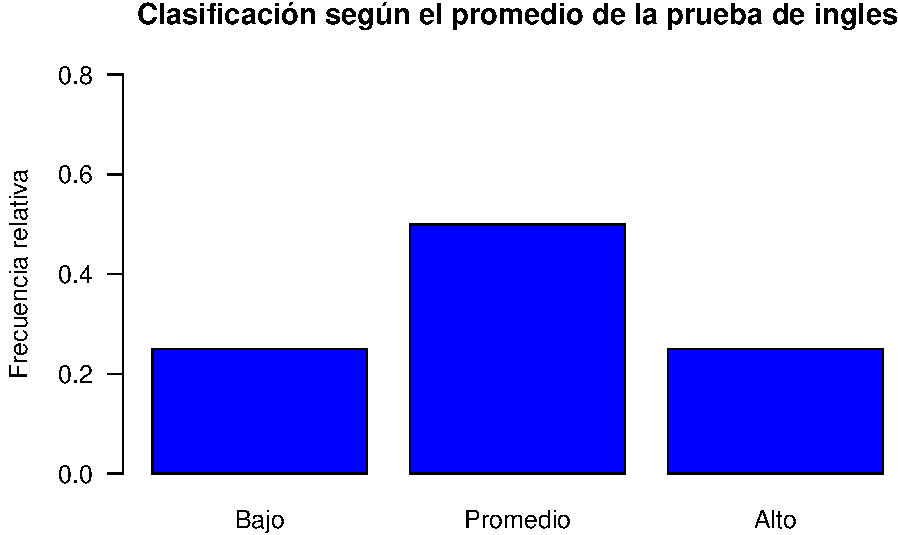
\includegraphics[width=0.95\linewidth]{figurasR/unnamed-chunk-18-1} \end{center}

\hypertarget{tabla-de-frecuencias-absolutas-por-2-variables}{%
\subsection{Tabla de frecuencias absolutas por 2
variables}\label{tabla-de-frecuencias-absolutas-por-2-variables}}

Analizaremos ahora dos variables la clasificación segun el promedio de
ingles y la naturaleza del colegio.
\begingroup\fontsize{8}{10}\selectfont

\begin{longtabu} to \linewidth {>{\raggedright}X>{\centering}X>{\centering}X>{\centering}X}
\caption{\label{tab:unnamed-chunk-19}Tabla de frecuencia absoluta por clasificacion puntaje prueba ingles y naturaleza del colegio.}\\
\toprule
 & Bajo & Promedio & Alto\\
\midrule
OFICIAL & 55 & 115 & 35\\
NO OFICIAL & 11 & 17 & 31\\
\bottomrule
\end{longtabu}
\endgroup{}

\hypertarget{tabla-de-frecuencias-relativas-por-2-variables}{%
\subsection{Tabla de frecuencias relativas por 2
variables}\label{tabla-de-frecuencias-relativas-por-2-variables}}

Analizaremos ahora dos variables la clasificación segun el promedio de
ingles y la naturaleza del colegio.
\begingroup\fontsize{8}{10}\selectfont

\begin{longtabu} to \linewidth {>{\raggedright}X>{\centering}X>{\centering}X>{\centering}X}
\caption{\label{tab:unnamed-chunk-20}Tabla de frecuencia relativa por clasificacion puntaje prueba ingles y naturaleza del colegio.}\\
\toprule
 & Bajo & Promedio & Alto\\
\midrule
OFICIAL & 0.2083 & 0.4356 & 0.1326\\
NO OFICIAL & 0.0417 & 0.0644 & 0.1174\\
\bottomrule
\end{longtabu}
\endgroup{}

\hypertarget{tabla-de-frecuencias-relativas-por-fila}{%
\subsection{Tabla de frecuencias relativas por
fila}\label{tabla-de-frecuencias-relativas-por-fila}}

Analizaremos ahora dos variables la clasificación segun el promedio de
ingles y la naturaleza del colegio.
\begingroup\fontsize{8}{10}\selectfont

\begin{longtabu} to \linewidth {>{\raggedright}X>{\centering}X>{\centering}X>{\centering}X}
\caption{\label{tab:unnamed-chunk-21}Tabla de frecuencia relativa por clasificacion puntaje prueba ingles y naturaleza del colegio.}\\
\toprule
 & Bajo & Promedio & Alto\\
\midrule
OFICIAL & 0.2683 & 0.5610 & 0.1708\\
NO OFICIAL & 0.1866 & 0.2881 & 0.5253\\
\bottomrule
\end{longtabu}
\endgroup{}

\hypertarget{grafico-frecuencias-absolutas-por-fila}{%
\subsection{Grafico frecuencias absolutas por
fila}\label{grafico-frecuencias-absolutas-por-fila}}

\begin{center}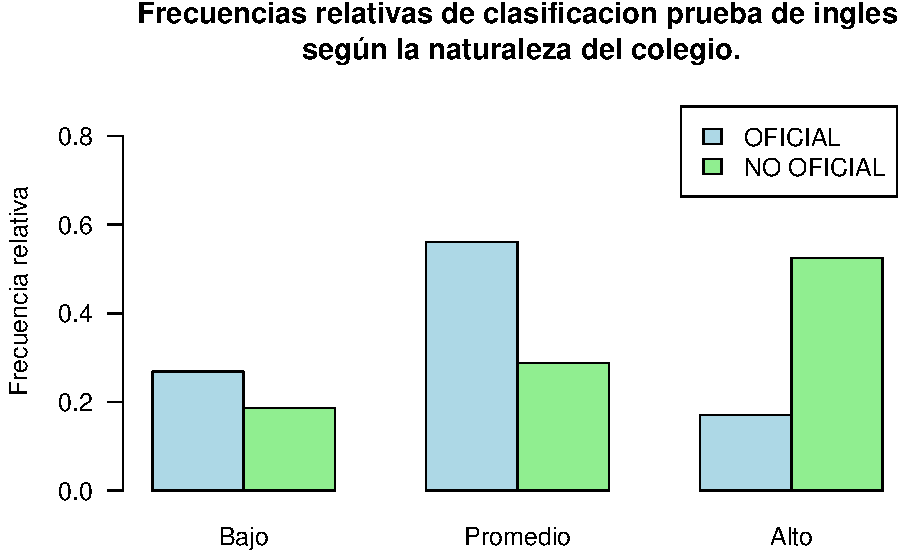
\includegraphics[width=0.95\linewidth]{figurasR/unnamed-chunk-22-1} \end{center}

\hypertarget{conclusiones}{%
\chapter{Conclusiones}\label{conclusiones}}

Después de analizar los datos, se observa una tendencia interesante en
cuanto al desempeño en las pruebas de inglés entre colegios oficiales y
no oficiales. Los colegios no oficiales muestran una mayor propensión a
obtener puntajes altos en la prueba de inglés en comparación con los
colegios oficiales. Específicamente, el 52.53\% de los estudiantes en
colegios no oficiales obtuvieron puntajes altos, mientras que solo el
17.08\% de los estudiantes en colegios oficiales lograron lo mismo.

Por otro lado, los colegios oficiales tienen una proporción más alta de
estudiantes con puntajes bajos en la prueba de inglés en comparación con
los colegios no oficiales. Un 26.83\% de los estudiantes en colegios
oficiales obtuvieron puntajes bajos, mientras que solo un 18.66\% de los
estudiantes en colegios no oficiales tuvieron resultados similares.

Estas conclusiones sugieren que el tipo de institución educativa puede
influir en el desempeño de los estudiantes en la prueba de inglés.
Aunque no se puede determinar la causa exacta de esta disparidad basada
únicamente en estos datos, es posible que los colegios no oficiales
tengan diferentes enfoques pedagógicos, recursos o condiciones que
contribuyan a un mejor rendimiento en inglés. Estos hallazgos podrían
ser útiles para informar políticas educativas y prácticas pedagógicas
destinadas a mejorar el aprendizaje del idioma inglés en colegios
oficiales. Sin embargo, se requiere una investigación más profunda para
comprender completamente los factores subyacentes detrás de esta
disparidad y desarrollar estrategias efectivas para abordarla.

\FloatBarrier

\ifdefined\ifprincipal
\else
\setlength{\parindent}{1em}
\pagestyle{fancy}
\setcounter{tocdepth}{4}
\tableofcontents

\fi

\ifdefined\ifdoblecara
\fancyhead{}{}
\fancyhead[LE,RO]{\scriptsize\rightmark}
\fancyfoot[LO,RE]{\scriptsize\slshape \leftmark}
\fancyfoot[C]{}
\fancyfoot[LE,RO]{\footnotesize\thepage}
\else
\fancyhead{}{}
\fancyhead[RO]{\scriptsize\rightmark}
\fancyfoot[LO]{\scriptsize\slshape \leftmark}
\fancyfoot[C]{}
\fancyfoot[RO]{\footnotesize\thepage}
\fi

\renewcommand{\headrulewidth}{0.4pt}
\renewcommand{\footrulewidth}{0.4pt}

\hypertarget{conclusiones-1}{%
\chapter{Conclusiones}\label{conclusiones-1}}

\hypertarget{generales}{%
\section{Generales}\label{generales}}

\begin{itemize}
\item
  xxxxxx
\item
  xxxxxxxxx
\item
  dsxxxxxxxx
\end{itemize}

\hypertarget{recomendaciones-futuras}{%
\section{Recomendaciones Futuras}\label{recomendaciones-futuras}}

\begin{itemize}
\item
  xxxxxx
\item
  xxxxxxxxx
\item
  dsxxxxxxxx
\end{itemize}

\FloatBarrier

\FloatBarrier
\cleardoublepage

\ifdefined\ifdoblecara
  \fancyhead[LE,RO]{}
  \fancyfoot[LO,RE]{}
  \fancyhead[CO,CE]{Bibliografía}
\else
  \fancyhead[RO]{}
  \fancyfoot[LO]{}
  \fancyhead[CO]{Bibliografía}
\fi

\ifdefined\ifcitapandoc

\hypertarget{bibliografuxeda}{%
\chapter*{Bibliografía}\label{bibliografuxeda}}
\addcontentsline{toc}{chapter}{Bibliografía}

\else

\nocite{RStudio,R-knitr,R-rmarkdown,knitr2015,knitr2014,rmarkdown2018,
rmarkdown2020}

\fi

\bibliography{bib/referencias.bib,bib/paquetes.bib}


\addcontentsline{toc}{chapter}{Bibliografía}


\end{document}
